% Created 2023-06-18 Sun 20:19
% Intended LaTeX compiler: pdflatex
\documentclass[11pt]{article}
\usepackage[utf8]{inputenc}
\usepackage[T1]{fontenc}
\usepackage{graphicx}
\usepackage{longtable}
\usepackage{wrapfig}
\usepackage{rotating}
\usepackage[normalem]{ulem}
\usepackage{amsmath}
\usepackage{amssymb}
\usepackage{capt-of}
\usepackage{hyperref}
\usepackage[2cm]{geometry}
\date{}
\title{Kalkulator statystyk postaci na potrzeby gry RPG Instrukcja}
\hypersetup{
 pdfauthor={},
 pdftitle={Kalkulator statystyk postaci na potrzeby gry RPG Instrukcja},
 pdfkeywords={},
 pdfsubject={},
 pdfcreator={Emacs 30.0.50 (Org mode 9.6.1)}, 
 pdflang={English}}
\begin{document}

\maketitle
\newpage
\section{Wymagania systemowe}
\label{sec:orgbc56e66}
\begin{itemize}
\item wxWidgets.
\item CMake.
\item System operacjny \href{https://wiki.archlinux.org/title/Arch\_Linux}{Arch linux} z menadżerem okien np. \href{https://hyprland.org/}{Hyprland}.
\end{itemize}
\section{Instalacja}
\label{sec:org9dabdf0}
Plik wykonywlany będzie znajdował się w akutalnym katalogu pod nazwą \texttt{app}. Należy uruchomić poniższy skrypt.
\begin{verbatim}
#!/bin/sh
git clone 'https://github.com/rafal11ck/PSK-INF-PROJ-programowanie-obiektowe-1.git' &&
cd PSK-INF-PROJ-programowanie-obiektowe-1/ &&
mkdir build &&
cd build &&
cmake ../src &&
cmake --build . --target app -j4 &&
cd frontRPG
\end{verbatim}
\newpage
\section{Obsługa}
\label{sec:org3cb56fc}
Podstawowymi danymi elementami kalkulatora są statystyki oraz sloty na ekwipunek. Należy zaczać ich dodania. Przy pomocy przycisków w zakładce \texttt{add} panelu \texttt{gamemaster}.
\begin{figure}[htbp]
\centering
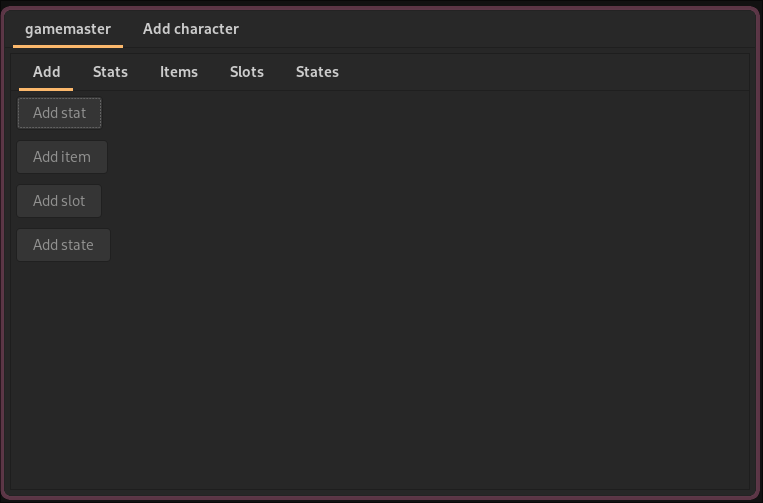
\includegraphics[width=.9\linewidth]{img/gamemaster.png}
\caption{Panel gamemaster.}
\end{figure}
\end{document}